\chapter{Suchen und Bearbeiten von Betriebsmitteln}
\label{Suchen und Bearbeiten von Betriebsmitteln}
Um den Inventardatensatz eines Betriebsmittels anzuzeigen, gen�gt es, die Seite Inventar->Suche zu �ffnen, und mithilfe des Barcodescanners den Strichcode einzuscannen. 
Die Betriebsmitteldaten werden automatisch angezeigt.
\begin{figure}
	\centering
	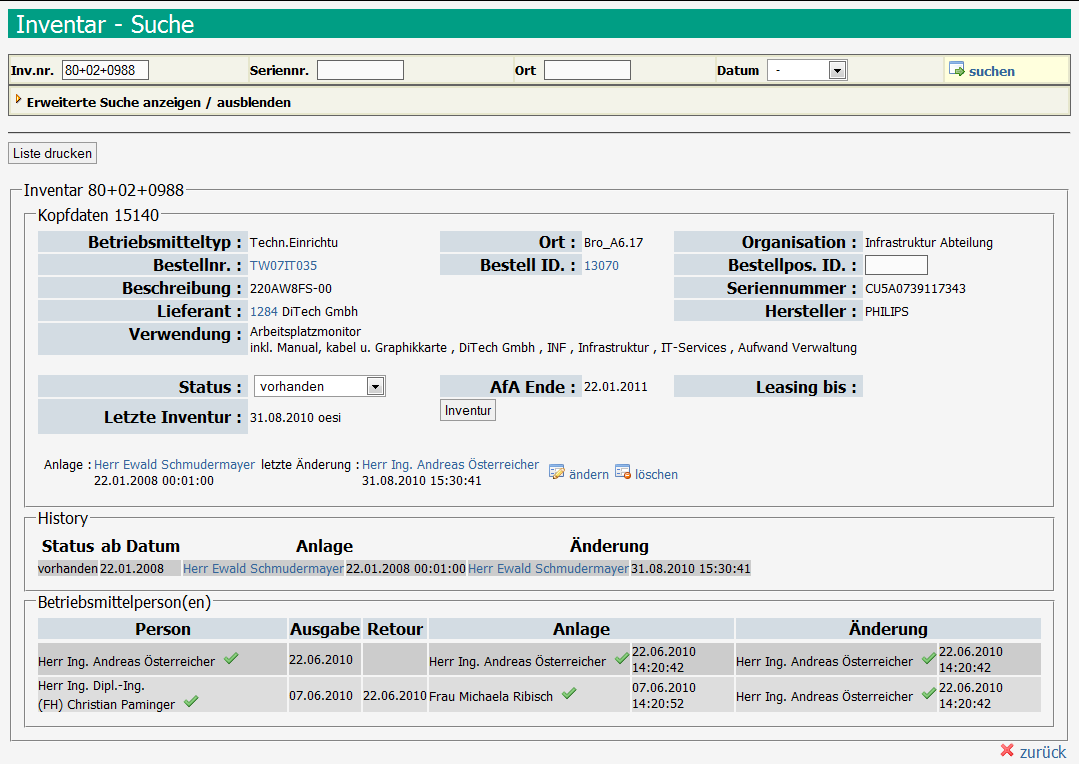
\includegraphics[width=0.80\textwidth]{Inventar_detail.png}
	\caption{Suche nach Betriebsmitteln}
	\label{Suche nach Betriebsmitteln}
\end{figure}

Betriebsmittel k�nnen auch nach Ort, Mitarbeiter, Organisationseinheit, etc gesucht werden.
Klicken Sie auf 'Erweiterte Suche anzeigen' um die Expertensuche einzublenden.

\begin{figure}
	\centering
	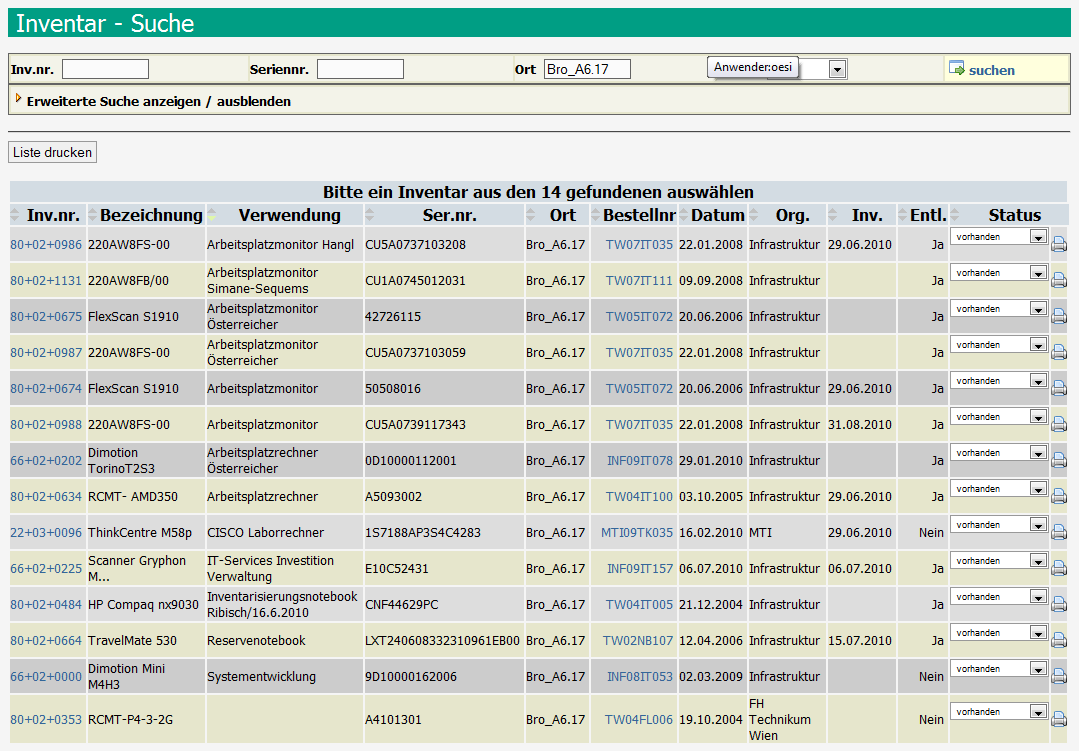
\includegraphics[width=0.80\textwidth]{Inventar_suche.png}
	\caption{Suche nach Betriebsmitteln}
	\label{Suche nach Betriebsmitteln}
\end{figure}

Um die Daten zu bearbeiten klicken Sie auf den Punkt '�ndern'.

\begin{figure}
	\centering
	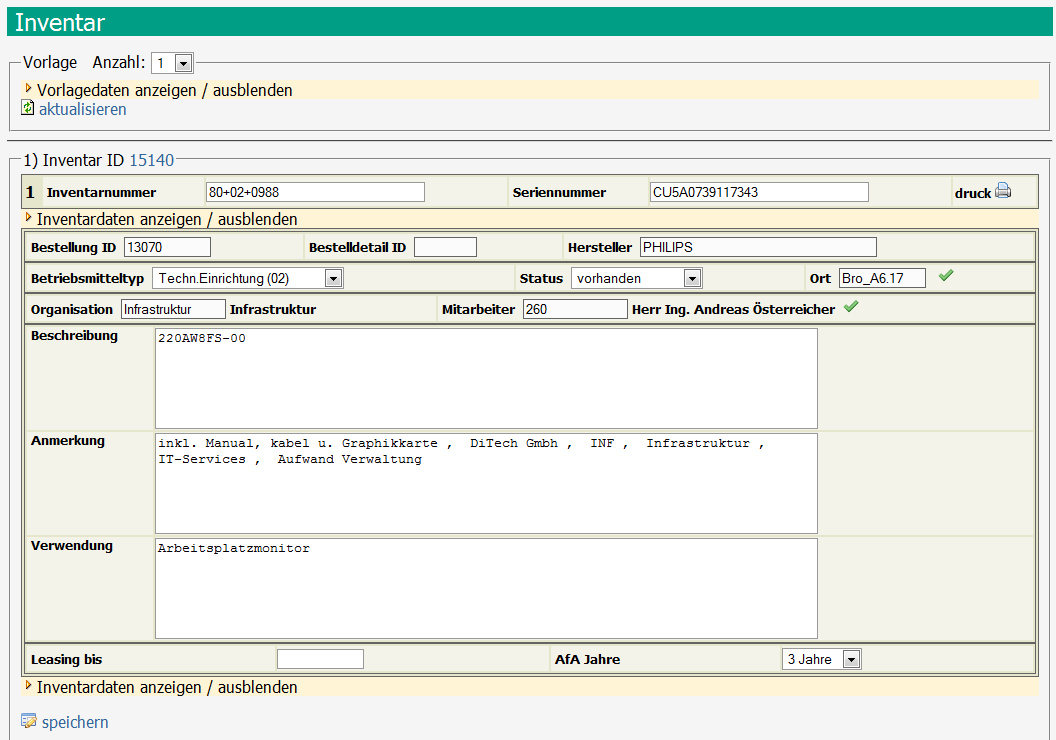
\includegraphics[width=0.80\textwidth]{Inventar_bearbeiten.png}
	\caption{�ndern von Betriebsmitteln}
	\label{�ndern von Betriebsmitteln}
\end{figure}